\documentclass[conference]{IEEEtran}
\IEEEoverridecommandlockouts
% The preceding line is only needed to identify funding in the first footnote.
% If that is unneeded, please comment it out.
\usepackage{cite}
\usepackage{amsmath,amssymb,amsfonts}
\usepackage{algorithmic}
\usepackage{graphicx}
\usepackage{textcomp}
\def\BibTeX{{\rm B\kern-.05em{\sc i\kern-.025em b}\kern-.08em
    T\kern-.1667em\lower.7ex\hbox{E}\kern-.125emX}}
\begin{document}

\title{Proposal\\
Blue-Collar Node : A Sharding Approach for Optimizing Storage on Blockchains
% Sharding for Blockchains Memory Optimization
% {\footnotesize \textsuperscript{*}Note: Sub-titles are not captured in Xplore and
% should not be used}
% \thanks{Identify applicable funding agency here. If none, delete this.}
}

\author{\IEEEauthorblockN{1\textsuperscript{st} Chawla}
\IEEEauthorblockA{\textit{Computer Science} \\
\textit{Arizona State University}\\
nchawla3@asu.edu}
\and
\IEEEauthorblockN{2\textsuperscript{nd} Saikia}
\IEEEauthorblockA{\textit{Computer Engineering} \\
\textit{Arizona State University}\\
csaikia@asu.edu}
}

\maketitle

\begin{abstract}
    The scalability of blockchain is a primary and urgent concern. The current
    popular blockchains have fundamental bottlenecks which limit their ability
    to have a higher throughput and a lower latency. One of the bottlenecks is
    the storage requirements of the current blockchains. All the full nodes and
    miners in a blockchain are required to store the complete blockchains and it
    grows everytime more transactions are added. The network relies mainly on
    commodity hardware for block propagation and transaction verification.
    With the increase in the size of blockchains, storing the entire blockchain
    on voluntary full nodes becomes impractical. Our project focuses at sharding
    this blockchain and storing it in several nodes. There is a two-fold advantage of this,
    transactions can be verified in parallel by different nodes and consensus
    can be achieved in a faster way increasing the throughput of the network,
    and the storage requirement of the full node will be decreased
    substantially. That directly will prevent the blockchain from getting
    centralized towards supercomputers. However, in this project we will focus
    only on the storage part of the problem. Executing transaction in parallel
    will be a part of the future work.
\end{abstract}

\begin{IEEEkeywords}
    blockchain, storage, sharding, blue-collar, decentralized
\end{IEEEkeywords}

\section{Introduction}
In 2009, Bitcoin\cite{bitcoin} introduced the first blockchain which is an
append only database that stores transactions. Blockchain maintains the
distributed database in a decentralized network aiming to solve the Byzantine
Generals Problem \cite{bgp}. Byzantine Generals Problem when extrapolated to
the banking system i.e to digital money translates to double spending problem,
where since there is no material money a malicious node can spend the money
twice, and since there is no central leader to check the money can be
spent.Bitcoin solves this problem by distributing the ledger to
every node in the network and cryptographically securing it making it immutable.
Special nodes called miners try to include the transactions into blocks by
solving a puzzle. This mechanism is called Proof of Work. Each miner then tries
to add this block to the distributed replicated ledger and after the block is
added each node on the network updates their ledger.

\subsection{Problems}
Satoshi Nakamoto randomly decided a block interval of 10 minutes between adding
2 blocks to the chain. The block size limited to 1MB. Since, the block size is
capped and the time interval is constant, the number of transactions that can be
dealt with are limited to ~3-7 transactions per second. 
Also, since the ledger is duplicated on each node on the network, as the ledger
grows the storage requirement of the node increases. 


\section{Background And Related Work}

\subsection{Background}
    Blockchain is a decentralized, tamper-proof digital ledger technology that
    is transforming transaction prospects for many industries. In addition to
    being the foundation of cryptocurrencies like Ethereum, the blockchain
    structure, which consists of linked blocks of information, allows for direct
    transactions across a network of computers without need for a central
    authority. The Ethereum network consists of three kind of nodes:
    \textbf{full nodes}, \textbf{light-weight nodes } and \textbf{miners}. Nodes
    save the complete blockchain and have two main functions: 
    \begin{enumerate}
        \item to validate transactions
        \item to propagate transactions and blocks in the network
    \end{enumerate} 
    Although full nodes validate transactions by checking their inputs and
    outputs, light clients verify transactions by SPV, or by requesting random
    chunks of a block and using the merkle root to verify each chunk. This
    verification technique relies on trust on a full node or the node sending
    data. This can be dangerous, because a malicious node can withhold small
    amount of data and can get unnoticed by many light clients. The network
    becomes much more trustworthy if the number of full nodes are a majority
    since data is always verified. As the blockchain technology is being adopted
    more, the storage requirement is increasing for each individual node. This
    increase in infrastructure requirement forces volunteer nodes to move to
    light-clients. This harms the network in 2 ways :
    \begin{enumerate}
        \item The network gets more centralized to people who can afford
            supercomputers
        \item The trust on the network weakens as most transactions are not
            completely validated by full nodes
    \end{enumerate}
    In this project, we want to introduce a new kind of node that saves only a
    part of the blockchain thus reducing the storage requirement and also
    validates each transaction that is a part of the block. This will introduce
    the following advantages to the network:
    \begin{enumerate}
        \item The trust on the network will be high as the nodes will validate
            each transaction fully.
        \item Randomizing block storage in such a way that transactions are
            fully validated by a small part of the network leading to multiple
            transactions being validated in parallel.
    \end{enumerate}
    We will be focusing only on the first advantage as a part of this project,
    the second would remain a future work.

\subsection{Related Work}
CRUSH\cite{crush} and RUSH\cite{rush} are used in a number of distributed storage
systems to handle the problem of data distribution by replication without
causing overhead on the network. The former uses a better approach but since the
replication factor is high in that algorithm, the blockchain might ultimately
store the same amount of data that it was storing earlier thus causing the
blue-collar nodes to store the same amount of data as a full node. We want to
change the algorithm to redirect the blocks to different nodes, but we want to
leverage the property of equal or balanced distribution form \cite{crush}.

"Sharding FAQ \cite{sharding} gives a good glimpse of the problem we are trying to
solve with techniques that will come in handy for us to make our solution
better.The difference in the approach is that \cite{sharding} tries to scale the
throughput of the blockchain while we focus on the storage optimization of the
system. 

"A note on data availability and erasure coding" \cite{erasure} is another blog by
the founder of Ethereum \cite{ethY}\cite{ethW} which touches our areas of concerns. It talks
about light clients and how their lack of validation techniques might be harmful
for the network. It exposes a loop-hole in the system which we want to remediate
by the creation of "blue-collar" nodes.

Elastico \cite{elastico} also attempted sharding but they also try to solve the
problem as discussed above i.e to have a higher throughput system.
\cite{elastico} also discusses centralized approaches of sharding in distributed
databases, some of them are Google's Spanner \cite{spanner}, Scatter
\cite{scatter}, and RSCoin \cite{rscoin}. These sharding protocols however do
not handle byzantine failures. 

\section{Proposed Solution}

\subsection{Components}
The key component of our system will be what we are calling a
\textbf{"Blue-collar node"}.
This node will be a combination of a light and full-node. This node will be
required to store the sharded blockchain and the parity bits such that if needed
it can re-create the data from a connected full node. \textbf{Data-distribution
algorithm} : Ceph utilizes CRUSH \cite{crush} (Controlled Replication Under
Scalable Hashing) which is a data distribution algorithm that distributes object
replicas across devices that belong to a heterogeneous storage cluster. In this
project, we want to focus in creating a variant of this algorithm, which doesn't
store replicas of objects (blocks in a blockchain) but stores only a part of the
blockchain and redirects the newly created block to only a part of nodes.
The algorithm should then create parity bits, that is different for each node
and helps each node create the blocks that are stored in other nodes when
any of the other nodes fail. To recreate this data we will be utilizing Erasure
Code\cite{erasure} and Reed-Solomon algorithm\cite{reed}.
\textbf{Monitor} : The monitor here will become a part of the ethereum protocol that
stores a map or DHT (Distributed Hash Table) of the data in its peer nodes and 
health of its peer nodes. 

\subsection{Architecture}
The current architecture of ethereum blockchain is shown in \ref{image: fig1}.
This architecture shows how in order to create Decentralized Application (dapp)
on Ethereum platform one needs to store the entire blockchain that is replicated
on both the instances (or all the instances). We intend on developing an
algorithm could be activated as a parameter to the ethereum protocol in a similar
fashion as light, fast or full node is activated. The new node type that we will
be adding is "blue-collar". This node will store part of the data and parity
bits calculated using the Reed-Solomon algorithm in order to re-create data on
another node when the node associated with the parity goes down.  

\begin{figure}
    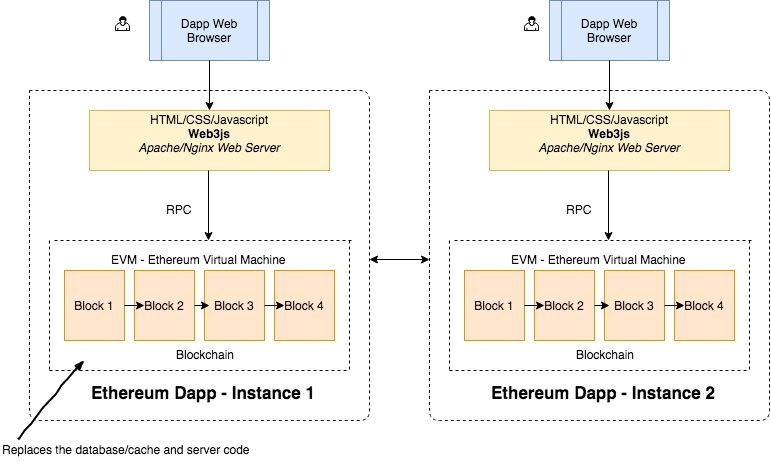
\includegraphics[width=.8\columnwidth]{files/ethArch.png}
    \centering
    \caption{Ethereum Architecture \cite{img} }
    \label{image: fig1}
\end{figure}

\subsection{Challenges}
In the methodology described above there are certain challenges that are not yet
handled. Some of them are listed below:

\begin{enumerate}
    \item The data distribution has to be randomized in such a way that a
        malicious intentions can't get hold of data that can be completely lost.
        In such a case, the contingency would be to recover the data from a full
        node and distribute it again over the network among peers but would
        require a lot of data movement.
    \item The data has to be distributed in such a way that in case some nodes
        fail, the re-distribution of data does not cause much data movement and
        doesn't occupy bandwidth that could be used for block propagation.
\end{enumerate}

\subsection{Implementation Plan}
We intend on using a container service to build a decentralized ditributed
network of Ethereum. There are multiple ready to use configurations that can be
utilized to run a private production ready Ethereum network.These available
container configurations automatically connect to the ethereum mainchain to run
a full node by running the default wallet. 
This can be used as a base system for us to implement our data-distribution
algorithm. This algorithm will have three variants suited for the three
different kinds of nodes on the network. 

\subsection{Evaluation Plan}
The proposed system would then be evaluated as to how much maximum storage is
required by the blue-collar node after we have sharded the blockchain. 
Metrics that will be used to evaluate the success of the project:
\begin{enumerate}
    \item Ratio of storage utilized by a full node to a blue-collar node
    \item Ratio of the bandwidth used by a full node to a blue-collar node
    \item Ratio of the bandwidth used by a light-client to a blue collar node
    \item Distribution of data among all the peer blue-collar nodes
    \item Data movement on blue-collar node failure
\end{enumerate}

\section{Proposed Schedule}
\begin{tabular}{|p{2cm}||p{2cm}||p{2cm}|}
    \hline
    \textbf{Task} & \textbf{Begin date} & \textbf{End date} \\
    \hline
    More literature survey & February 1st,2018 & February 13th, 2018 \\
    \hline
    Setting up the Ethereum system on Docker or Kubernetes & February 14th, 2018 & February 28th, 2018 \\
    \hline
    Testing scenarios for Ethereum Blockchain & March 1st, 2018 & March 
    7th, 2018 \\
    \hline
    Creating the data distribution algorithm & February 15th, 2018 & March 15th, 2018 \\
    \hline
    Monitor & March 16th, 2018 & March 31st, 2018 \\
    \hline
    Testing & April 1st, 2018 & End Sem \\
    \hline
\end{tabular}

\begin{thebibliography}{00}
    \bibitem{crush} Weil, S. A., Brandt, S. A., Miller, E. L., \& Maltzahn, C.
        (2006, November). CRUSH: Controlled, scalable, decentralized placement
        of replicated data. In Proceedings of the 2006 ACM/IEEE conference on
        Supercomputing (p. 122). ACM.
    \bibitem{erasure} Buterin, Vitalik. "A note on data availability and erasure coding"
        Github. https://github.com/ethereum/research/wiki/A-note-on-data-availability-and-erasure-coding
        Accessed 2nd January, 2018 . 
    \bibitem{sharding} Zamyatin, Alexie. "Sharding FAQ" Github.
        https://github.com/ethereum/wiki/wiki/Sharding-FAQ
        Accessed 2nd January, 2018
    \bibitem{elastico} Luu, L., Narayanan, V., Zheng, C., Baweja, K., Gilbert, S., \&
        Saxena, P. (2016, October). A secure sharding protocol for open
        blockchains. In Proceedings of the 2016 ACM SIGSAC Conference on
        Computer and Communications Security (pp. 17-30). ACM.
    \bibitem{img} Zastrin. https://www.zastrin.com/courses/1/lessons/2-3
    \bibitem{rush} Honicky, R. J., \& Miller, E. L. (2004, April). Replication
        under scalable hashing: A family of algorithms for scalable
        decentralized data distribution. In Parallel and Distributed Processing
        Symposium, 2004. Proceedings. 18th International (p. 96). IEEE.
    \bibitem{bitcoin} Nakamoto, Satoshi. "Bitcoin: A peer-to-peer electronic cash
        system." (2008).
    \bibitem{ethY} Wood, Gavin. "Ethereum: A secure decentralised generalised
        transaction ledger." Ethereum Project Yellow Paper 151 (2014): 1-32.
    \bibitem{ethW} Buterin, Vitalik. "Ethereum white paper." GitHub repository
        (2013).
    \bibitem{erasure} Dimakis, A. G., Godfrey, P. B., Wu, Y., Wainwright, M. J., &
        Ramchandran, K. (2010). Network coding for distributed storage systems.
        IEEE transactions on information theory, 56(9), 4539-4551.
    \bibitem{reed} Reed, I. S., \& Solomon, G. (1960). Polynomial codes over
        certain finite fields. Journal of the society for industrial and applied
        mathematics, 8(2), 300-304.
    \bibitem{spanner} James C. Corbett, Jeffrey Dean, Michael Epstein, Andrew
        Fikes, Christopher Frost, J. J. Furman, Sanjay Ghemawat,
        Andrey Gubarev, Christopher Heiser, Peter Hochschild, Wilson Hsieh,
        Sebastian Kanthak, Eugene Kogan, Hongyi Li, Alexander Lloyd, Sergey
        Melnik, David Mwaura, David Nagle, Sean Quinlan, Rajesh Rao, Lindsay
        Rolig, Yasushi Saito, Michal Szymaniak, Christopher Taylor, Ruth Wang,
        and Dale Woodford. Spanner: Google’s globally distributed database. ACM
        Trans. Comput. Syst., aug 2013.
    \bibitem{scatter} Lisa Glendenning, Ivan Beschastnikh, Arvind Krishnamurthy,
        and Thomas Anderson. Scalable consistency in scatter. In Proceedings of
        the Twenty-Third ACM Symposium on Operating Systems Principles, SOSP
        ’11, pages 15–28, New York, NY, USA, 2011. ACM.
    \bibitem{rscoin} Jonathan Katz, Andrew Miller, and Elaine Shi.
        Pseudonymous broadcast and secure computation from cryptographic
        puzzles. Cryptology ePrint Archive, Report 2014/857, 2014.
        http://eprint.iacr.org/2014/857.
    \bibitem{bgp} Lamport, L., Shostak, R., & Pease, M. (1982). The Byzantine
        generals problem. ACM Transactions on Programming Languages and Systems
        (TOPLAS), 4(3), 382-401.
\end{thebibliography}

\end{document}
